\documentclass[a4paper,11pt,dvipdfmx]{jsarticle}


% 数式
\usepackage{amsmath,amsfonts}
\usepackage{bm}

% 画像
\usepackage[dvipdfmx]{graphicx}
\usepackage{framed}

% 図形
\usepackage{tikz}
\usepackage{circuitikz}
\usepackage[utf8]{inputenc}
\usepackage{geometry}
\geometry{margin=2cm}
\usetikzlibrary{shapes.geometric}
\usetikzlibrary {shapes.misc}

% ソースコード
\usepackage{listings,jlisting,color}
\lstset{
basicstyle={\ttfamily},
identifierstyle={\small},
commentstyle={\smallitshape},
keywordstyle={\small\bfseries},
ndkeywordstyle={\small},
stringstyle={\small\ttfamily},
frame={tb},
breaklines=true,
columns=[l]{fullflexible},
numbers=left,
xrightmargin=0zw,
xleftmargin=3zw,
numberstyle={\scriptsize},
stepnumber=1,
numbersep=1zw,
lineskip=-0.5ex
}
\renewcommand{\lstlistingname}{ソースコード}

\usepackage{booktabs}
\usepackage{pgfplots}
\pgfplotsset{compat=1.18} % 最新の互換性を指定
\usepackage{here}


\begin{document}
\definecolor{shadecolor}{gray}{0.70}

\begin{titlepage}
\noindent
\vspace{4cm}
\begin{center}
\begin{LARGE}
組込システムI \\
第9回  課題 \\
\vspace{8cm}
提出日  2025/06/19 \\
学籍番号  21T2166D \\
名前  渡辺 大樹 \\
\end{LARGE}
\end{center}
\end{titlepage}
\setcounter{page}{1}

\section{演習(1)}
\subsection{課題}
2つの温度センサ、アナログのLM35DZとデジタルのADT7410を同時に接続し、それぞれの計測値を摂氏(°C)単位で比較する。アナログセンサはA/DコンバータMCP3002を介してSPI通信で、デジタルセンサはI2C通信で読み取る。

\subsection{使用部品}
\begin{itemize}
    \item Raspberry Pi 4B
    \item アナログ温度センサ (LM35DZ)
    \item デジタル温度センサ (ADT7410)
    \item A/Dコンバータ (MCP3002)
    \item ブレッドボード
    \item ジャンパー線
\end{itemize}

\subsection{回路図と回路写真}
\begin{figure}[H]
    \centering
    \begin{circuitikz}[american, scale=0.9, every node/.style={scale=0.8}]
        % Raspberry Pi
        \draw[thick] (0,0) rectangle (3,6);
        \node[font=\bfseries] at (1.5,6.3) {\textbf{Raspberry Pi 4B}};
        \node[anchor=west] at (0,5.5) {+3.3V}; \node[anchor=east] at (0.1, 5.5) {Pin 1};
        \node[anchor=west] at (0,5) {SDA}; \node[anchor=east] at (0.1, 5) {Pin 3};
        \node[anchor=west] at (0,4.5) {SCL}; \node[anchor=east] at (0.1, 4.5) {Pin 5};
        \node[anchor=west] at (0,3.5) {MOSI}; \node[anchor=east] at (0.1, 3.5) {Pin 19};
        \node[anchor=west] at (0,3) {MISO}; \node[anchor=east] at (0.1, 3) {Pin 21};
        \node[anchor=west] at (0,2.5) {SCLK}; \node[anchor=east] at (0.1, 2.5) {Pin 23};
        \node[anchor=west] at (0,2) {CE0}; \node[anchor=east] at (0.1, 2) {Pin 24};
        \node[anchor=west] at (0,0.5) {GND}; \node[anchor=east] at (0.1, 0.5) {Pin 6};
        
        % Power lines
        \draw[red, thick] (3,5.5) -- (10,5.5) node[above,pos=0.5] {+3.3V};
        \draw[black, thick] (3,0.5) -- (10,0.5) node[below,pos=0.5] {GND};

        % ADT7410 (I2C)
        \draw (5,4.5) node[dipchip, num pins=4, external pins width=0.1] (adt7410) {ADT7410};
        \node[anchor=east, scale=0.7] at (adt7410.pin 1) {SDA};
        \node[anchor=east, scale=0.7] at (adt7410.pin 2) {SCL};
        \node[anchor=west, scale=0.7] at (adt7410.pin 3) {$V_{DD}$};
        \node[anchor=west, scale=0.7] at (adt7410.pin 4) {$V_{SS}$};
        \draw (3,5) -- (adt7410.pin 1); % SDA
        \draw (3,4.5) -- (adt7410.pin 2); % SCL
        \draw (adt7410.pin 3) |- (9,5.5); % VDD
        \draw (adt7410.pin 4) |- (5,0.5); % VSS/GND

        % MCP3002 (SPI)
        \node (mcp3002) [dipchip, num pins=8, external pins width=0.3] at (7,2) {MCP3002};
        \node[anchor=east, scale=0.7] at (mcp3002.pin 1) {CS/SHDN};
        \node[anchor=east, scale=0.7] at (mcp3002.pin 2) {CH0};
        \node[anchor=east, scale=0.7] at (mcp3002.pin 3) {CH1};
        \node[anchor=east, scale=0.7] at (mcp3002.pin 4) {$V_{SS}$/GND};
        \node[anchor=west, scale=0.7] at (mcp3002.pin 5) {$D_{IN}$/SDI};
        \node[anchor=west, scale=0.7] at (mcp3002.pin 6) {$D_{OUT}$/SDO};
        \node[anchor=west, scale=0.7] at (mcp3002.pin 7) {CLK};
        \node[anchor=west, scale=0.7] at (mcp3002.pin 8) {$V_{DD}$/$V_{REF}$};

        \draw (3,2) -- (5.5, 2) |- (mcp3002.pin 1); % CS/SHDN
        \draw (3,3.5) -- (mcp3002.pin 5); % MOSI
        \draw (3,3) -- (mcp3002.pin 6); % MISO
        \draw (3,2.5) -- (mcp3002.pin 7); % SCLK
        \draw (mcp3002.pin 8) |- (9,5.5); % VDD/VREF
        \draw (mcp3002.pin 4) |- (7,0.5); % VSS/GND
        
        % LM35DZ
        \draw (11,2) node[op amp, noinv input up] (lm35dz) {};
        \node at (10,3) {LM35DZ};
        \draw (lm35dz.out) |- ++(0, -1.2) -- ++(-6.5, 0) |- (mcp3002.pin 2);
        \draw (lm35dz.+) |- (10,5.5);
        \draw (lm35dz.-) |- (10,0.5);
    \end{circuitikz}
    \caption{演習(1)の回路図}
    \label{fig:circuit1}
\end{figure}
\begin{figure}[H]
    \centering
    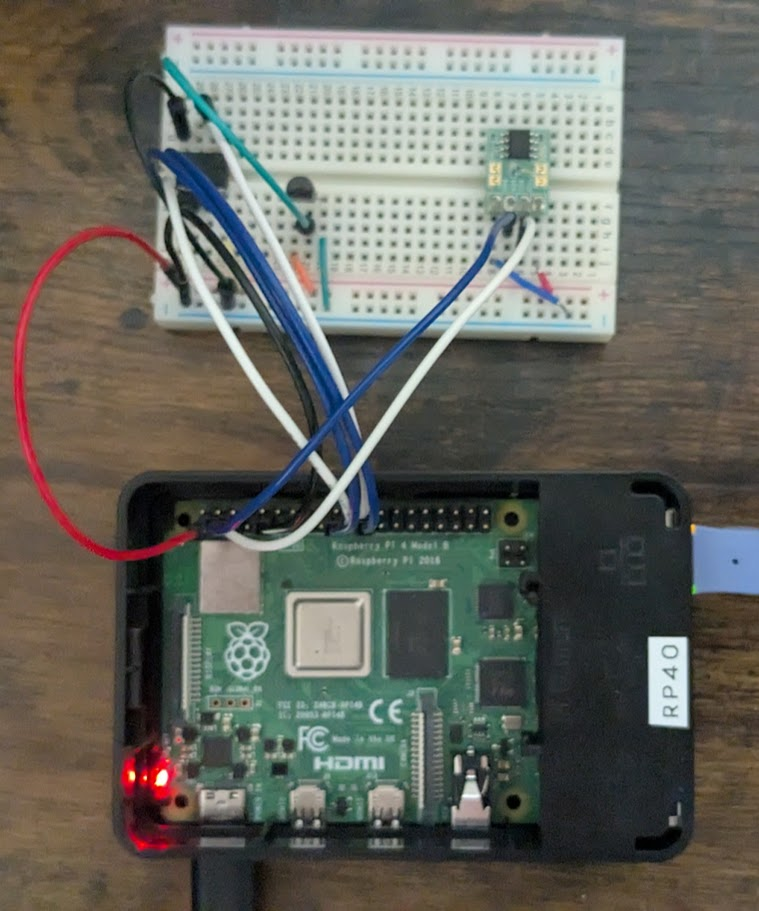
\includegraphics[width=0.7\textwidth]{img/9-1.png}
    \caption{演習(1)の回路写真}
    \label{fig:photo1}
\end{figure}

\subsection{アルゴリズムの説明}
\begin{enumerate}
    \item I2CバスとSPIバスをそれぞれ初期化する。ADT7410のアドレスは0x48、MCP3002はSPIデバイス0(CE0)に設定する。
    \item `read\_adt7410`関数でI2C通信を行い、ADT7410から温度データを読み取る。2バイトのデータを結合し、13bitの2の補数表現として解釈した後、分解能0.0625を乗じて温度に変換する。
    \item `read\_mcp9700a`関数でSPI通信を行い、MCP3002のCH0からA/D変換値を取得する。得られた10bitのデジタル値を電圧に変換し、温度係数(10.0mV/°C)を用いて温度に変換する。LM35DZは0°Cで0Vを出力するため、オフセットの計算は不要である。
    \item メインループ内で1秒ごとに両方のセンサから温度を取得し、コンソールに表示する。
\end{enumerate}

\subsection{結果}
プログラムを実行し、2つの温度センサの値を異なる時間帯で計測した。
\begin{verbatim}
# 2025/06/19 18:20
# ADT7410 (Digital): 27.56 C, LM35DZ (Analog): 27.42 C
# ADT7410 (Digital): 27.50 C, LM35DZ (Analog): 27.10 C
# ADT7410 (Digital): 28.12 C, LM35DZ (Analog): 27.10 C
# ADT7410 (Digital): 27.94 C, LM35DZ (Analog): 27.42 C
# ADT7410 (Digital): 29.00 C, LM35DZ (Analog): 27.42 C

# 2025/06/19 19:20
# ADT7410 (Digital): 27.56 C, LM35DZ (Analog): 26.45 C
# ADT7410 (Digital): 26.94 C, LM35DZ (Analog): 26.45 C
# ADT7410 (Digital): 27.50 C, LM35DZ (Analog): 26.45 C
# ADT7410 (Digital): 27.50 C, LM35DZ (Analog): 26.45 C
# ADT7410 (Digital): 27.06 C, LM35DZ (Analog): 26.13 C
# ADT7410 (Digital): 26.75 C, LM35DZ (Analog): 26.45 C
\end{verbatim}

\subsection{考察}
18:20の計測では、指でセンサを温めたため、両方のセンサで温度上昇が観測された。ADT7410の方がLM35DZよりも値の変動が大きく、より敏感に反応しているように見える。19:20の計測では、室温が安定しているため両者の値は近くなったが、ADT7410の方が若干高い値を示した。これは、ADT7410の精度が±0.5°Cであるのに対し、LM35DZは代表的な精度が±1°C程度であるためと考えられる。デジタルセンサはノイズに強く、より正確な値を提供する傾向があることが確認できた。

\section{演習(2)}
\subsection{課題}
SPI通信のチップセレクト機能を利用して、2つのSPIデバイス(A/DコンバータMCP3002と3軸加速度センサLIS3DH)を同時に制御する。温度と加速度の値を同時に取得し、表示する。

\subsection{使用部品}
\begin{itemize}
    \item Raspberry Pi 4B
    \item アナログ温度センサ (LM35DZ)
    \item 3軸加速度センサ (LIS3DH)
    \item A/Dコンバータ (MCP3002)
    \item ブレッドボード
    \item ジャンパー線
\end{itemize}

\subsection{回路図と回路写真}
\begin{figure}[H]
    \centering
    \begin{circuitikz}[american, scale=0.9, every node/.style={scale=0.8}]
        % Raspberry Pi
        \draw[thick] (0,0) rectangle (3,6);
        \node[font=\bfseries] at (1.5,6.3) {Raspberry Pi 4B};
        \node[anchor=east] at (0,5.5) {+3.3V};
        \node[anchor=east] at (0,4.5) {MOSI};
        \node[anchor=east] at (0,4) {MISO};
        \node[anchor=east] at (0,3.5) {SCLK};
        \node[anchor=east] at (0,3) {CE0};
        \node[anchor=east] at (0,2.5) {CE1};
        \node[anchor=east] at (0,0.5) {GND};
        
        % Power lines
        \draw[red, thick] (3,5.5) -- (12,5.5) node[above] {+3.3V};
        \draw[black, thick] (3,0.5) -- (12,0.5) node[below] {GND};

        % MCP3002 (SPI CE0)
        \draw (6,2) node[draw, rectangle, minimum width=1.5cm, minimum height=1cm] (mcp3002) {};
        \node at (6.75,2.7) {MCP3002};
        \draw (3,3) -- (mcp3002.west |- 0,3); % CE0
        \draw (3,4) -- (mcp3002.west |- 0,4); % MISO
        \draw (3,4.5) -- (mcp3002.west |- 0,4.5); % MOSI
        \draw (3,3.5) -- (mcp3002.west |- 0,3.5); % SCLK
        \draw (mcp3002.north) -- (mcp3002.north |- 0,5.5);
        \draw (mcp3002.south) -- (mcp3002.south |- 0,0.5);

        % LM35DZ
        \draw (8,1.5) node[op amp, noinv input up] (lm35dz) {};
        \node at (8,2.5) {LM35DZ};
        \draw (lm35dz.out) -- (mcp3002.east);
        \draw (lm35dz.up) -- (8,5.5);
        \draw (lm35dz.down) -- (8,0.5);

        % LIS3DH (SPI CE1)
        \draw (10,4) node[draw, rectangle, minimum width=1.5cm, minimum height=1cm] (lis3dh) {};
        \node at (10.75,4.7) {LIS3DH};
        \draw (3,2.5) -- (lis3dh.west |- 0,2.5); % CE1
        \draw (3,4) -- (lis3dh.west |- 0,4); % MISO
        \draw (3,4.5) -- (lis3dh.west |- 0,4.5); % MOSI
        \draw (3,3.5) -- (lis3dh.west |- 0,3.5); % SCLK
        \draw (lis3dh.north) -- (lis3dh.north |- 0,5.5);
        \draw (lis3dh.south) -- (lis3dh.south |- 0,0.5);
    \end{circuitikz}
    \caption{演習(2)の回路図}
    \label{fig:circuit2}
\end{figure}
\begin{figure}[H]
    \centering
    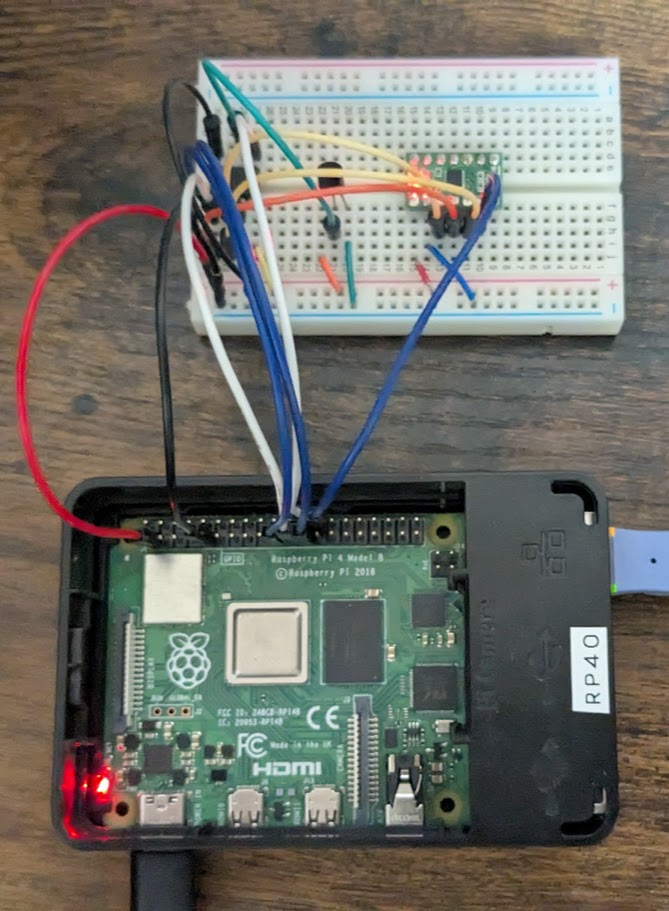
\includegraphics[width=0.7\textwidth]{img/9-2.png}
    \caption{演習(2)の回路写真}
    \label{fig:photo2}
\end{figure}

\subsection{アルゴリズムの説明}
\begin{enumerate}
    \item `spidev`のインスタンスを2つ生成し、それぞれデバイス0(CE0)とデバイス1(CE1)に割り当てる。
    \item `setup\_lis3dh`関数で、LIS3DHのCTRL\_REG1(0x20)に0x27を書き込み、データレート10Hz、XYZ軸有効のノーマルモードに設定する。
    \item `read\_lis3dh\_axis\_g`関数で、指定された軸のレジスタから2バイト読み取り、12bitの2の補数データに変換後、g単位の加速度に変換する。
    \item メインループ内で10秒ごとに、CE0に接続されたMCP3002から温度を、CE1に接続されたLIS3DHから3軸の加速度を読み取り、コンソールに表示する。
\end{enumerate}

\subsection{結果}
プログラムを実行し、温度と加速度を同時にモニタリングした。センサを静止させた状態ではZ軸が約1gを示し、傾けると重力加速度が各軸に分散される様子が確認できた。
\begin{verbatim}
# Temp: 27.42 C | Accel X: 0.007, Y: 0.035, Z: 1.059
# Temp: 27.42 C | Accel X: 0.007, Y: 0.027, Z: 1.066
# (センサをX軸方向に傾けた場合)
# Temp: 26.45 C | Accel X: -0.781, Y: 0.121, Z: 0.680
# (センサをY軸方向に傾けた場合)
# Temp: 26.77 C | Accel X: -0.050, Y: 1.047, Z: 0.058
\end{verbatim}

\subsection{考察}
SPIバスを共有しながら、CE0とCE1を切り替えることで2つの異なるデバイスを独立して制御できることを確認した。`spidev`ライブラリがこの切り替えを抽象化しているため、プログラム上では異なるインスタンスを操作するだけで簡単に実現できた。これにより、少ないピン数で多くのデバイスを接続できるSPIの利点を実感した。加速度センサの値をg単位に変換する計算では、データシートから分解能やデータ形式を正確に読み取ることの重要性を学んだ。

\section{演習(3)}
\subsection{課題}
演習(2)のシステムにLEDを追加し、温度または加速度が設定した閾値を超えた場合に、LEDを点滅させて異常を通知するシステムを構築する。

\subsection{使用部品}
\begin{itemize}
    \item Raspberry Pi 4B
    \item アナログ温度センサ (LM35DZ)
    \item 3軸加速度センサ (LIS3DH)
    \item A/Dコンバータ (MCP3002)
    \item LED (赤色)
    \item 抵抗 (330Ω)
    \item ブレッドボード
    \item ジャンパー線
\end{itemize}

\subsection{回路図と回路写真}
\begin{figure}[H]
    \centering
    \begin{circuitikz}[american, scale=0.9, every node/.style={scale=0.8}]
        % Raspberry Pi
        \draw[thick] (0,0) rectangle (3,6.5);
        \node[font=\bfseries] at (1.5,6.8) {Raspberry Pi 4B};
        \node[anchor=east] at (0,6) {+3.3V};
        \node[anchor=east] at (0,5) {MOSI};
        \node[anchor=east] at (0,4.5) {MISO};
        \node[anchor=east] at (0,4) {SCLK};
        \node[anchor=east] at (0,3.5) {CE0};
        \node[anchor=east] at (0,3) {CE1};
        \node[anchor=east] at (0,2) {GPIO21};
        \node[anchor=east] at (0,0.5) {GND};
        
        % Power lines
        \draw[red, thick] (3,6) -- (12,6) node[above] {+3.3V};
        \draw[black, thick] (3,0.5) -- (12,0.5) node[below] {GND};

        % LED
        \draw (3,2) to[short] (4,2) to[R, l=330$\Omega$] (4,1) to[led, l=LED] (4,0.5);

        % MCP3002 (SPI CE0)
        \draw (6,2.5) node[draw, rectangle, minimum width=1.5cm, minimum height=1cm] (mcp3002) {};
        \node at (6.75,3.2) {MCP3002};
        \draw (3,3.5) -- (mcp3002.west |- 0,3.5); % CE0
        \draw (3,4.5) -- (mcp3002.west |- 0,4.5); % MISO
        \draw (3,5) -- (mcp3002.west |- 0,5); % MOSI
        \draw (3,4) -- (mcp3002.west |- 0,4); % SCLK
        \draw (mcp3002.north) -- (mcp3002.north |- 0,6);
        \draw (mcp3002.south) -- (mcp3002.south |- 0,0.5);

        % LM35DZ
        \draw (8,2) node[op amp, noinv input up] (lm35dz) {};
        \node at (8,3) {LM35DZ};
        \draw (lm35dz.out) -- (mcp3002.east);
        \draw (lm35dz.up) -- (8,6);
        \draw (lm35dz.down) -- (8,0.5);

        % LIS3DH (SPI CE1)
        \draw (10,4.5) node[draw, rectangle, minimum width=1.5cm, minimum height=1cm] (lis3dh) {};
        \node at (10.75,5.2) {LIS3DH};
        \draw (3,3) -- (lis3dh.west |- 0,3); % CE1
        \draw (3,4.5) -- (lis3dh.west |- 0,4.5); % MISO
        \draw (3,5) -- (lis3dh.west |- 0,5); % MOSI
        \draw (3,4) -- (lis3dh.west |- 0,4); % SCLK
        \draw (lis3dh.north) -- (lis3dh.north |- 0,6);
        \draw (lis3dh.south) -- (lis3dh.south |- 0,0.5);
    \end{circuitikz}
    \caption{演習(3)の回路図}
    \label{fig:circuit3}
\end{figure}
\begin{figure}[H]
    \centering
    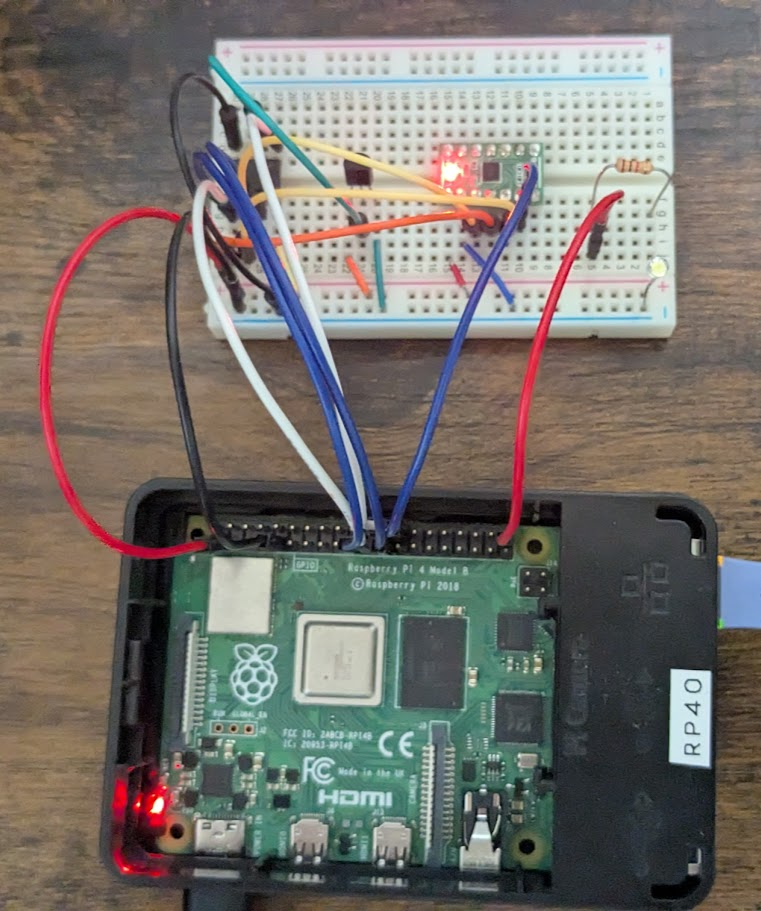
\includegraphics[width=0.7\textwidth]{img/9-3.png}
    \caption{演習(3)の回路写真}
    \label{fig:photo3}
\end{figure}

\subsection{アルゴリズムの説明}
\begin{enumerate}
    \item 演習(2)のコードをベースに、`RPi.GPIO`ライブラリを追加し、LEDを接続したGPIO21を出力モードに設定する。
    \item 温度の閾値(30.0°C)と加速度の閾値(1.5g)を定数として定義する。
    \item メインループの周期を0.5秒に短縮し、よりリアルタイムに異常を検知できるようにする。
    \item 温度が閾値を超えた場合、「TEMPERATURE ALERT」と表示し、LEDを0.1秒間隔で5回点滅させる。
    \item 加速度のいずれかの軸の絶対値が閾値を超えた場合、「ACCELERATION ALERT」と表示し、LEDを0.3秒間隔で3回点滅させる。
    \item 正常時はLEDを消灯状態に保つ。
    \item KeyboardInterrupt発生時に、GPIOとSPIのクリーンアップ処理を行う。
\end{enumerate}

\subsection{結果}
プログラムを実行し、センサを手で温めたり、振ったりして異常状態を発生させた。
\begin{verbatim}
# (温度を30℃以上に上げた場合)
# Temp: 30.32 C | Accel X: 0.003, Y: 0.042, Z: 1.066
!!! TEMPERATURE ALERT !!!
# (LEDが速く5回点滅)

# (加速度を1.5g以上に上げた場合)
# Temp: 27.42 C | Accel X: 0.429, Y: 0.062, Z: 1.993
!!! ACCELERATION ALERT !!!
# (LEDが遅く3回点滅)
\end{verbatim}
結果として、温度と加速度の異常をそれぞれ異なる点滅パターンで正しく通知できることを確認した。

\subsection{考察}
本演習では、センサからの入力に応じて出力を制御する、組込システムの基本的なフィードバックループを実装した。センサの値に基づいて条件分岐を行い、GPIOを操作することで、単なるデータロガーから一歩進んだ実用的なアプリケーションを構築できた。異常の種類によってLEDの点滅パターンを変えることで、ユーザーは視覚的にどのセンサが異常を検知したかを判断できる。これは、より高度なHMI(Human Machine Interface)の基礎となる考え方である。ポーリング周期を0.5秒に設定したが、これは検知のリアルタイム性とCPU負荷のトレードオフであり、実際の製品開発では要求仕様に応じて最適な値を決定する必要があると感じた。

\section{問いの解答}
\textbf{問い:演習(1)において、氷点下10度のときのAD変換器の出力値(10bit)と、ADT7410の出力値(13bit)を計算で求めなさい.}

\textbf{解答:}
\subsection{LM35DZとMCP3002 (A/D変換器)}
LM35DZの仕様より、温度係数は10.0mV/°Cであり、0°Cでの出力電圧は0mVである。
-10°Cのときの出力電圧 $V_{out}$ は、
\begin{equation}
V_{out} = 0 \text{mV} + (10.0 \text{mV/°C} \times -10 \text{°C}) = -100 \text{mV} = -0.1 \text{V}
\end{equation}
しかし、MCP3002の入力電圧範囲はGNDからVdd(3.3V)までであり、負の電圧を直接測定することはできない。したがって、回路が負電圧を扱えるように設計されていない限り、-10°Cのときの入力電圧はGNDレベル(0V)として読み取られる。
\begin{equation}
D_{ADC} = \frac{0 \text{V}}{3.3 \text{V}} \times 1023 = 0
\end{equation}
したがって、この回路構成におけるAD変換器の出力値は \textbf{0} となる。

\subsection{ADT7410 (デジタル温度センサ)}
ADT7410の仕様より、13bitモードでの温度分解能は0.0625°Cである。
-10°Cのときのデジタル出力値 $D_{ADT}$ は、
\begin{equation}
D_{ADT} = \frac{-10 \text{°C}}{0.0625 \text{°C/LSB}} = -160
\end{equation}
この値は13bitの2の補数で表現される。
正の160は、13bitバイナリで `000 1010 0000` となる。
-160を求めるには、全ビットを反転して1を加える。
\begin{enumerate}
    \item 全ビット反転: `111 0101 1111`
    \item 1を加算: `111 0110 0000`
\end{enumerate}
したがって、ADT7410の出力値は16進数で \textbf{0x1D80}、2進数で \textbf{`11101100000`} となる。

\newpage
\section{付録:ソースコード}
\subsection{演習(1)のソースコード}
\lstinputlisting[label=Python1, caption=exam9-1.py]{C:/Program_Code/Python/BuiltIn/9/exam9-1.py}

\subsection{演習(2)のソースコード}
\lstinputlisting[label=Python2, caption=exam9-2.py]{C:/Program_Code/Python/BuiltIn/9/exam9-2.py}

\subsection{演習(3)のソースコード}
\lstinputlisting[label=Python3, caption=exam9-3.py]{C:/Program_Code/Python/BuiltIn/9/exam9-3.py}

\end{document}
